\chapter{Compilación y arara}
Para generar los índices la compilación debe ser:
\begin{flushleft}
  \verb|lualatex MiDocumento.tex|\\
  \verb|makeindex MiDocumento.idx|\\
  \verb|lualatex MiDocumento.tex|
\end{flushleft}

Para ser más precisos se debería correr \texttt{makeindex} en cada índice que
se haya creado. En nuestro documento debería ser en el documento principal,
como arriba, para formar al índice alfabético y en \texttt{names.idx} para
formar el índice de nombres.

Si se considera la cadena de compilación que se generará cuando se tomé en
cuenta la de la sección~\ref{sec:bib} para generar la bibliografía ahora
resulta en
\begin{flushleft}
  \verb|lualatex MiDocumento.tex|\\
  \verb|biber MiDocumento|\\
  \verb|makeindex MiDocumento.idx|\\
  \verb|lualatex MiDocumento.tex|\\
  \verb|lualatex MiDocumento.tex|
\end{flushleft}
Como claramente tiene más pasos puede que haga el proceso algo lento. Para
hacer más rápida la compilación hay que evitar los pasos innecesarios. Las
primeras líneas del archivo principal son de la forma
\begin{flushleft}
  \verb|% arara: ...|
\end{flushleft}
las uso para compilar con \texttt{arara} ya que se pueden agregar
condicionales de manera sencilla. Al menos mucho más simple que crear un
\texttt{latexmk} o un \texttt{makefile}. Aunque seguramente su instalación
local sí debe incluir \texttt{arara}, desgraciadamente overleaf no incluye
esta opción e ignorará los \textit{magic comments} del principio del archivo.

Con estos comandos sólo compilará la bibliografía cuando sea necesario, la
primera vez y cuando se modifiqué la bibliografía. De la misma forma sólo
compilara el índice alfabético cuando haga falta. En la primera compilación
de \texttt{lualatex} sólo creara los archivos auxiliares, ganando así un
poco de tiempo y las siguientes veces que corra \texttt{lualatex} activará
la opción \texttt{synctex} para que su editor y visor se comuniquen.

Ahora se compila con el comando
\begin{flushleft}
  \verb|arara MiDocumento|
\end{flushleft}
Para mostrar cómo mejoró el tiempo de compilación la segunda
vez pongo capturas de pantalla de la compilación de este documento.
Además muchos editores de \LaTeX{} pueden configurarse para compilar con
\texttt{arara}.  Por ejemplo, en Atom (el editor que uso) con el paquete atom-
latex se configura como \textit{custom toolchain} y el toolchain es:
\begin{flushleft}
  \verb|arara %DOC -v|
\end{flushleft}
como se explica en \url{https://github.com/ashthespy/Atom-LaTeX}.
\begin{figure}
  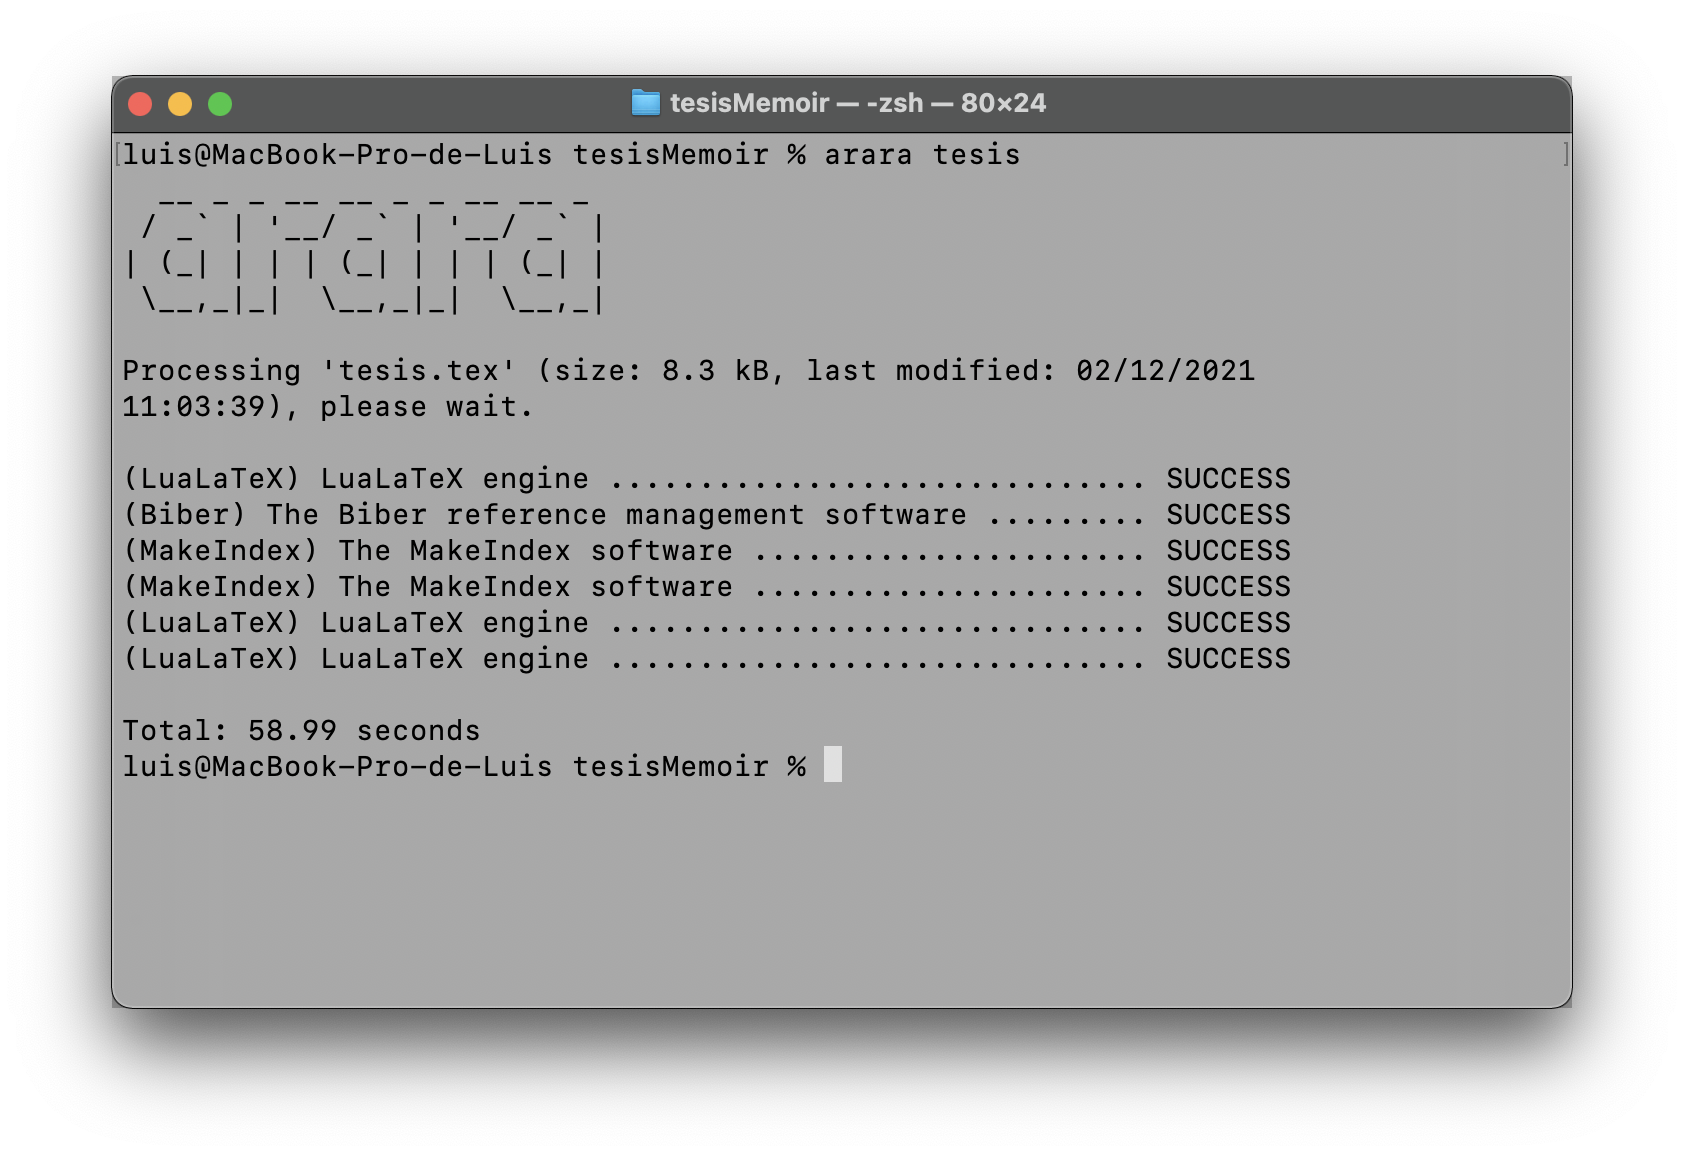
\includegraphics[scale=0.3]{primera}
  \caption{Primera compilación}
\end{figure}

\begin{figure}
  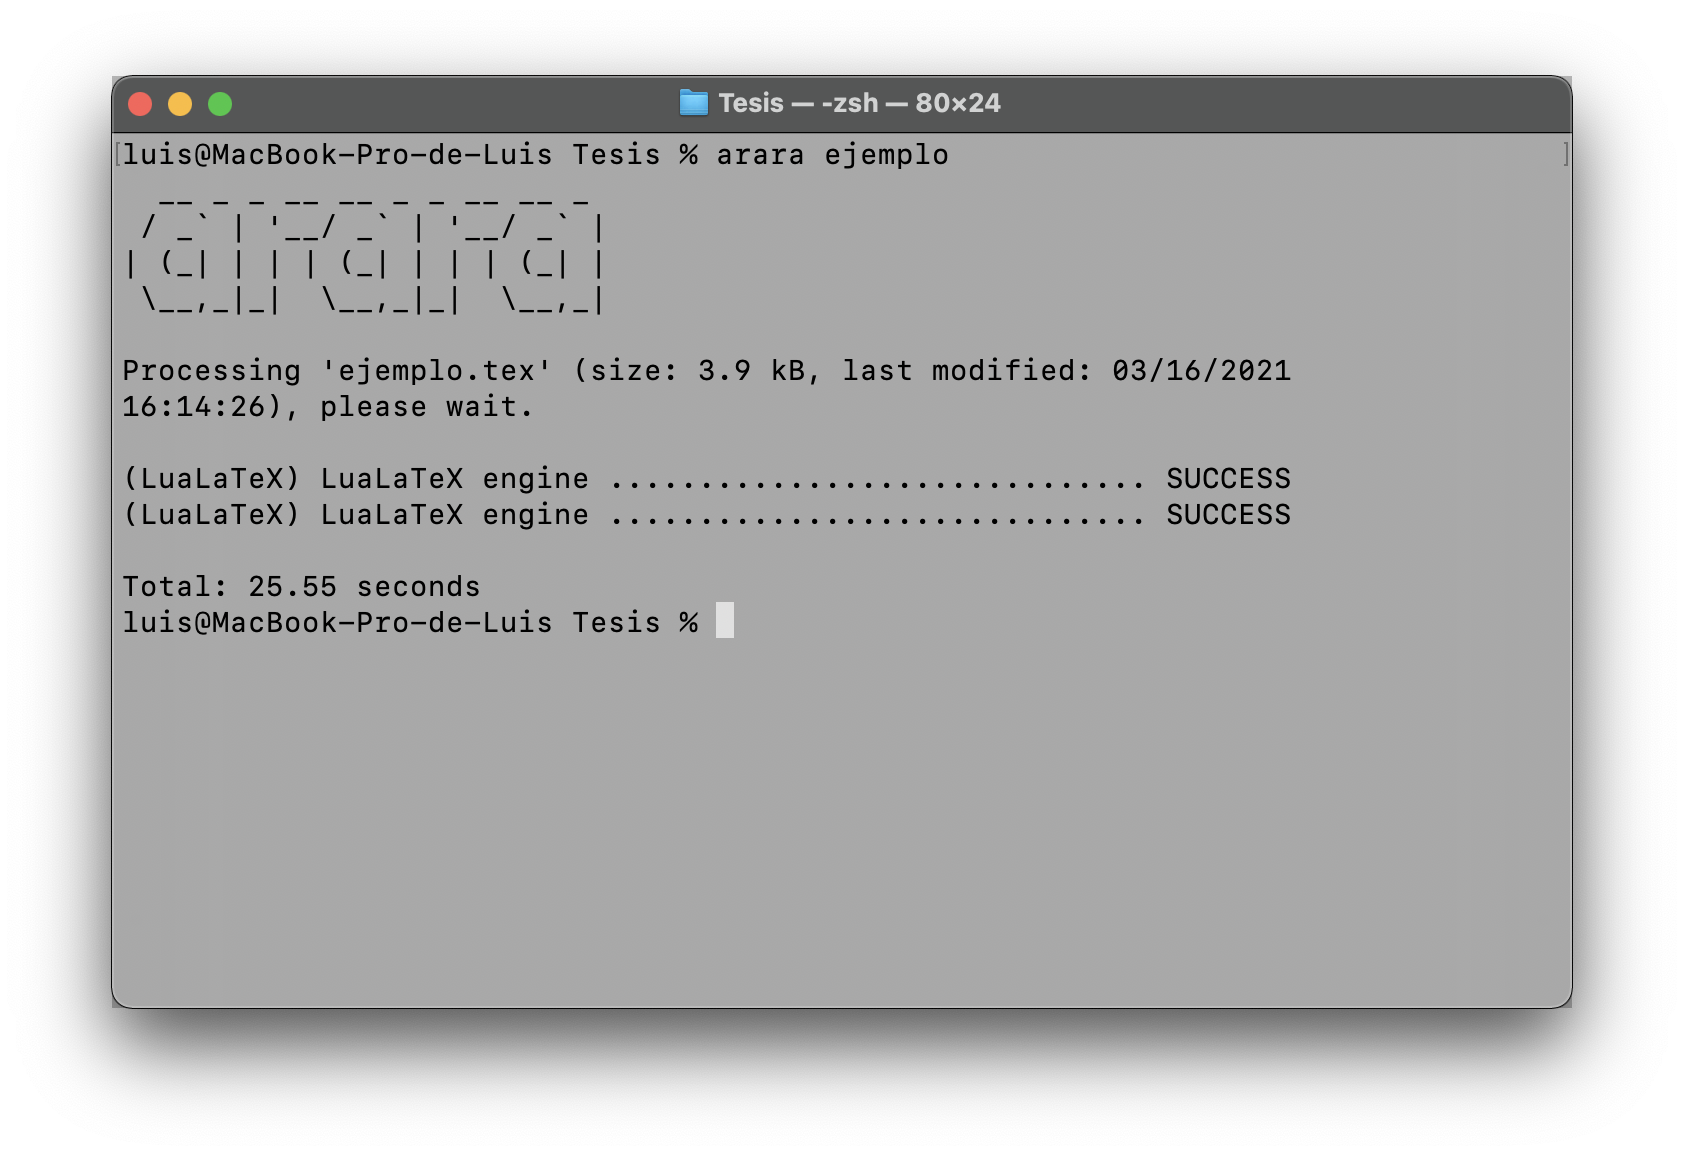
\includegraphics[scale=0.3]{segunda}
  \caption{Segunda compilación}
\end{figure}

Para configurarlo en TeXMaker hay que seguir las instrucciones en
\url{https://tex.stackexchange.com/a/107995}.

En TeXWorks: \url{https://tex.stackexchange.com/a/98795}.

En TeXShop: \url{https://tex.stackexchange.com/a/175673}.
